\documentclass{template_svk}

\usepackage[utf8]{inputenc}
\usepackage[czech]{babel}
\usepackage{url}

\def\mtt#1{{\footnotesize\tt#1}}
\def\comm#1{\mtt{\char92#1}}

\begin{document}

\title{Detekce příjmu karbohydrátů diabetického pacienta 1. typu}

% Autoři
 \author{David Pivovar}{student navazujícího studijního programu Inženýrská informatika, obor Medicínská informatika, specializace Projektant a správce medicínských IS, e-mail: pivovar@students.zcu.cz}

\maketitle

\section{Úvod}

Diabetes mellitus je rozšířené chronické metabolické onemocnění. Vyznačuje se zvýšenou koncentrací cukru v krvi (glykémie), která vniká z nedostatku inzulinu nebo rezistencí vůči jeho působení. Hlavní součástí léčby je monitorace koncentrace glukózy a podávání inzulinu. V dnešní době je možné sledovat vývoj glykémie díky sytémům kontinuální monitorace glukózy (CGMS) a kontinuálnímu dávkování inzulinu inzulinovou pumpou. Integrace těchto dvou systémů umožňuje autonomní řízení dávkování inzulinu v závislosti na aktuální koncentraci glukózy. Jedním z takových systémů je SmartCGMS \citep{smartcgms} vyvíjený na katedře Informatiky a výpočetní techniky.

Příjem karbohydrátů (jídla) značně ovlivňuje koncentraci glukózy v krvi. Na to musí být systém schopen reagovat podáním dávky inzulinu. V současné době zadává pacient přijaté karbohydráty do SmartCGMS sám. Cílem této práce je vytvořit modul do SmartCGMS pro detekci příjmu karbohydrátů z dat CGMS.

\section{Detekce příjmu karbohydrátů}

\cite{turksoy} navrhli algoritmus detekce na základě rychlosti výskytu glukózy za použití Bergmanova minimálního modelu. Podobný postup zvolili \cite{hyunjin} a vytvořili hlasovací schéma, kdy jsou vysílány impulsy pokud první a druhá derivace intersticiální glukózy překročí sérii thresholdů.

Nově navržená metoda detekuje vzestupné a klesající hrany průběhu intersticiální glukózy pomocí thresholdů první diference měřených hodnot intersticiální glukózy. Data intersticiální glukózy, která jsou senzorem měřena v pětiminutových intervalech, jsou před samotným výpočtem vyhlazena pomocí Savitzky-Golay filtru \citep{savgol}.

Derivace funkce $f'(x)$ v bodě $x$ je směrnicí tečny funkce $f(x)$ v daném bodě. Pakliže je funkce $f(x)$ v bodě $x$ rostoucí, je její směrnice tečny v bodě $x$ kladná. Pokud je $f(x)$ klesající, její směrnice tečny je v daném místě záporná. Velikost derivace v bodě $x$ pak udává velikost změny $f(x)$, neboli říká, jak strmě funkce stoupá či klesá. Derivace funkce $f(x)$ v bodě $x_{1}$ můžeme vyjádřit jako:
\begin{equation}
f'(x) = \frac{d}{dx}f(x) = \lim_{x \to x_{0}} \frac{f(x)-f(x_{0})}{x-x_{0}}
\end{equation}

Jelikož data ze senzoru CGMS jsou diskrétní, můžeme derivaci nahradit rovnicí první diference. Pro data intersticiální glukózy tak dostáváme vztah:
\begin{equation}
\Delta IST = \frac{IST_{t} - IST_{t-1}}{\Delta t}
\end{equation}

Následně se data ohodnotí. Pokud $\Delta IST$ překročí určitý threshold $th_{i}$, přiřadí se váha $w_{i}$. Takových dvojic thresholdů a vah může být libovolné množství. Experimentálně byla zjištěna kombinace thresholdů $th=[0.0125, 0.018]$ a vah $w=[2.25, 3]$. Por určení vývoje křivky v čase se ohodnocení dat zvyšuje v případě, že předchozí hodnoty vykazují vzrůstající trend po dobu dvou hodin nazpět (tj. 24 hodnot). Získá se tak aktivační funkce pro rostoucí hrany. Pro klesající hrany se použije stejný postup, ale se záporným ohodnocením.

Aby byl detekován příjem karbohydrátů, musí být aktivační funkce rostoucí hrany alespoň 3 (nízká  pravděpodobnost). Pokud aktivační funkce překročí hodnotu 5.5, je příjem detekován s vysokou pravděpodobností.

Uváděné hodnoty parametrů jsou experimentální a lze je v systému SmartCGMS změnit individuálně pro každého pacienta.

\section{Výsledky}

Detekce hran je na obrázku \ref{obr}.

\begin{figure}[!ht]
  \centering
  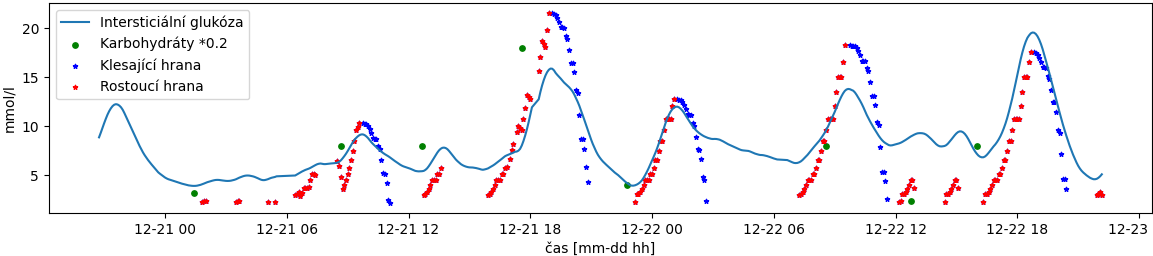
\includegraphics[width=1\textwidth]{hrany2}
  \caption{Detekce hran průběhu intersticiální glukózy}
  \label{obr}
\end{figure}

Algoritmus byl otestován na datech jedenácti pacientů. Měření u každého pacienta probíhalo po dobu 10 - 11 dnů. V součtu pacienti zaznamenali 340 jídel za 109 dnů. Počet detekovaných jídel navrženým algoritmem byl 289 (85 \%), z čehož 167 (57,8 \%) jídel bylo potvrzeno s vysokou pravděpodobností. Falešně pozitivních detekcí bylo 112. To může být dáno tím, že pacienti nezadávali jídla poctivě nebo je zadávali se zpožděním. Také prudké výkyvy hladiny cukru v krvi spojené s jinou činností mohou způsobit falešnou detekci. Průměrné zpoždění detekce bylo 27,54 minuty, což je srovnatelné, nebo i lepší než výsledky ostatních algoritmů. 


\begin{thebibliography}{99}\itemsep=.75ex%

\bibitem[Koutný et al. (2020)]{smartcgms}
Koutny, T., Ubl, M. SmartCGMS as a Testbed for a Blood-Glucose Level Prediction and/or Control Challenge with (an FDA-Accepted)Diabetic Patient Simulation. Procedia Computer Science. 2020, 177, s. 354–362. ISSN 1877-0509.

\bibitem[Hyunjin et al. (2020)]{hyunjin}
Hyunjin, L. P. et al. A Closed-Loop Artificial Pancreas Using Model Predictive Control and a Sliding Meal Size Estimator. Journal of Diabetes Science and Technology. sep 2009, 3, 5, s. 1082–1090. 

\bibitem[Turksoy et al. (2020)]{turksoy}
Turksoy, K. et al. Real-time insulin bolusing for unannounced meals with artificial pancreas. Control Engineering Practice. 2017, 59, s. 159–164. ISSN 0967-0661.

\bibitem[Luo et al. (2020)]{savgol}
 Luo, J., Ying, K., Bai, J. Savitzky–Golay smoothing and differentiation filter for even number data. Signal Processing. 2005, 85, 7, s. 1429–1434. ISSN 0165-1684. 

\end{thebibliography}

\end{document}
